\documentclass{article}%[12pt, a4paper]{article}

\usepackage{ucs}
\usepackage[russian]{babel}
\usepackage{cmap}
\usepackage[utf8x]{inputenc}
\usepackage{amsthm}
\usepackage{amsmath}
\usepackage{amssymb}
\usepackage{graphicx}
\usepackage{float}
\usepackage{clrscode}
\usepackage{tocloft}
\usepackage[usenames]{color}
\usepackage[margin=20mm]{geometry}
\usepackage{sidecap}
\usepackage{url}
\usepackage{hyperref}

\frenchspacing



\begin{document}

\begin{titlepage}

\begin{center}

\large Санкт-Петербургский Государственный Политехнический Университет \\
Кафедра <<Прикладная математика>> \\ [8.0cm]
\textbf{\textsc{ОТЧЕТ ПО ЛАБОРАТОРНОЙ РАБОТЕ №4}}\\[1.0cm]
По курсу ``Операционные системы''\\[3.0cm]

\begin{minipage}{0.4\textwidth}
\begin{flushleft} \large
  Выполнил студент гр. 4057/2: \\ [1.0cm]
  Преподаватель:
\end{flushleft}
\end{minipage}
\begin{minipage}{0.4\textwidth}
\begin{flushright} \large
Зенцев Ф.К. \\ [1.0cm]
Тимофеев Д.А.
\end{flushright}
\end{minipage}

\vfill

\large Санкт-Петербург 2010



\end{center}
\end{titlepage}


\renewcommand{\cftsecleader}{\cftdotfill{\cftsubsecdotsep}}

\onecolumn

\tableofcontents

\onecolumn

\section{Введение}

\noindent
Летнюю производственную практику я провёл за решением нескольких задач, потребовавшихся
для проекта, посвященного распознаванию химических структур. В качестве введения проясню предназначение
такого проекта.\\

\noindent
Существует достаточно много различного рода программных продуктов, разработанных для нужд специалистов в области химии:
редакторы молекул, системы поиска молекул в базах данных, системы моделирования химических реакций. Такое программное 
обеспечение работает с некоторым машинным представлением молекул. В машинном приближении молекулы, химические структуры 
cуть помеченные неориентированные графы, где метки вершин это названия атомов, а рёбер - различные
виды связей: одинарная, двойная, тройная, стереосвязь. \\

\begin{figure}[h]
\centering
{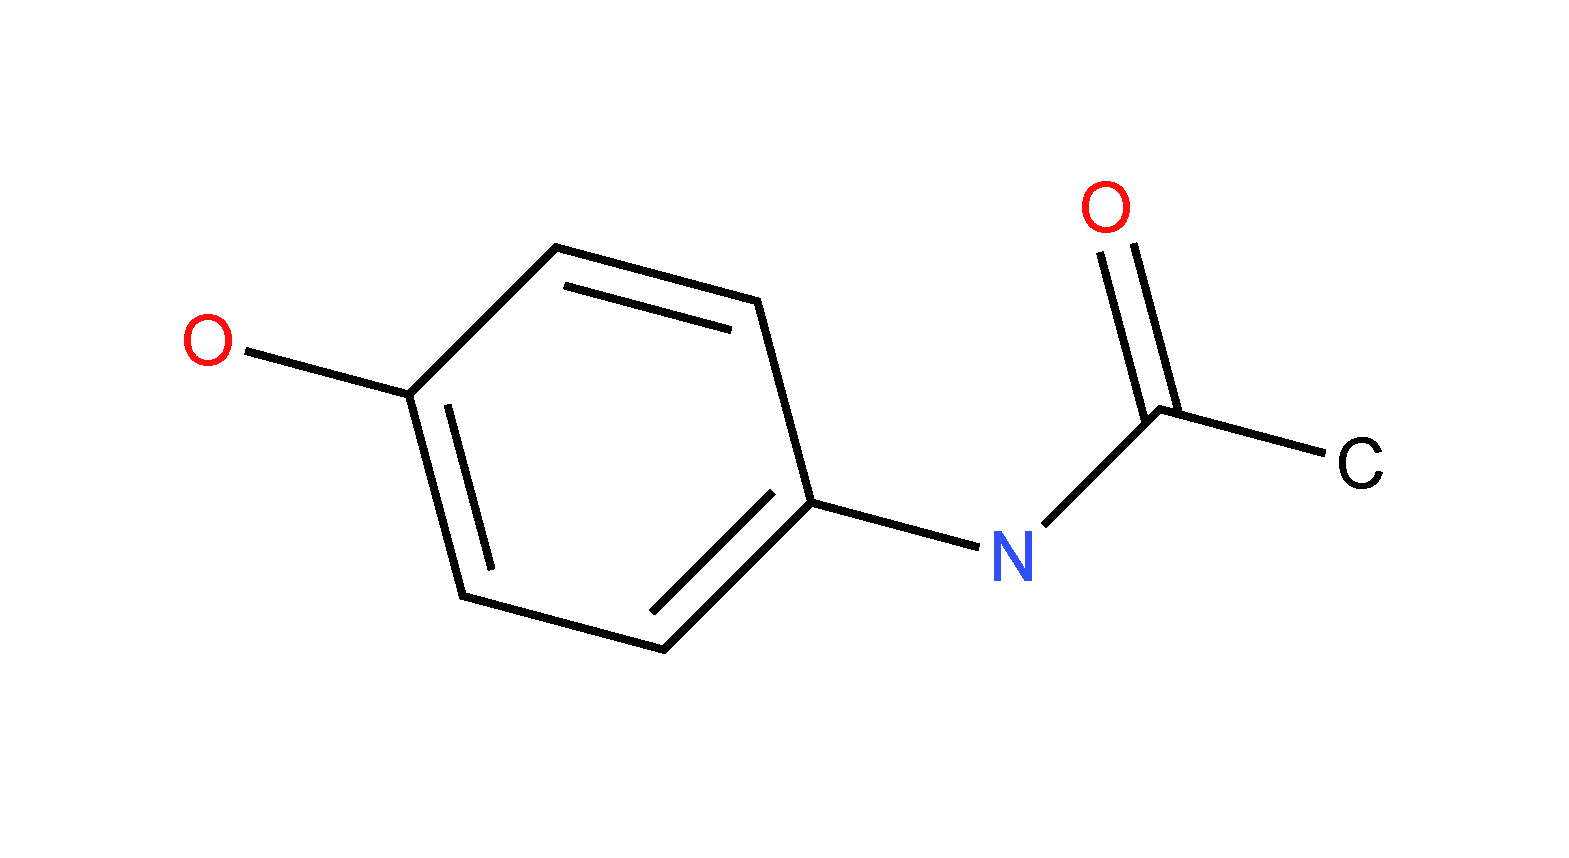
\includegraphics[width=0.35\textwidth]{img/paracetomolum.pdf}}
{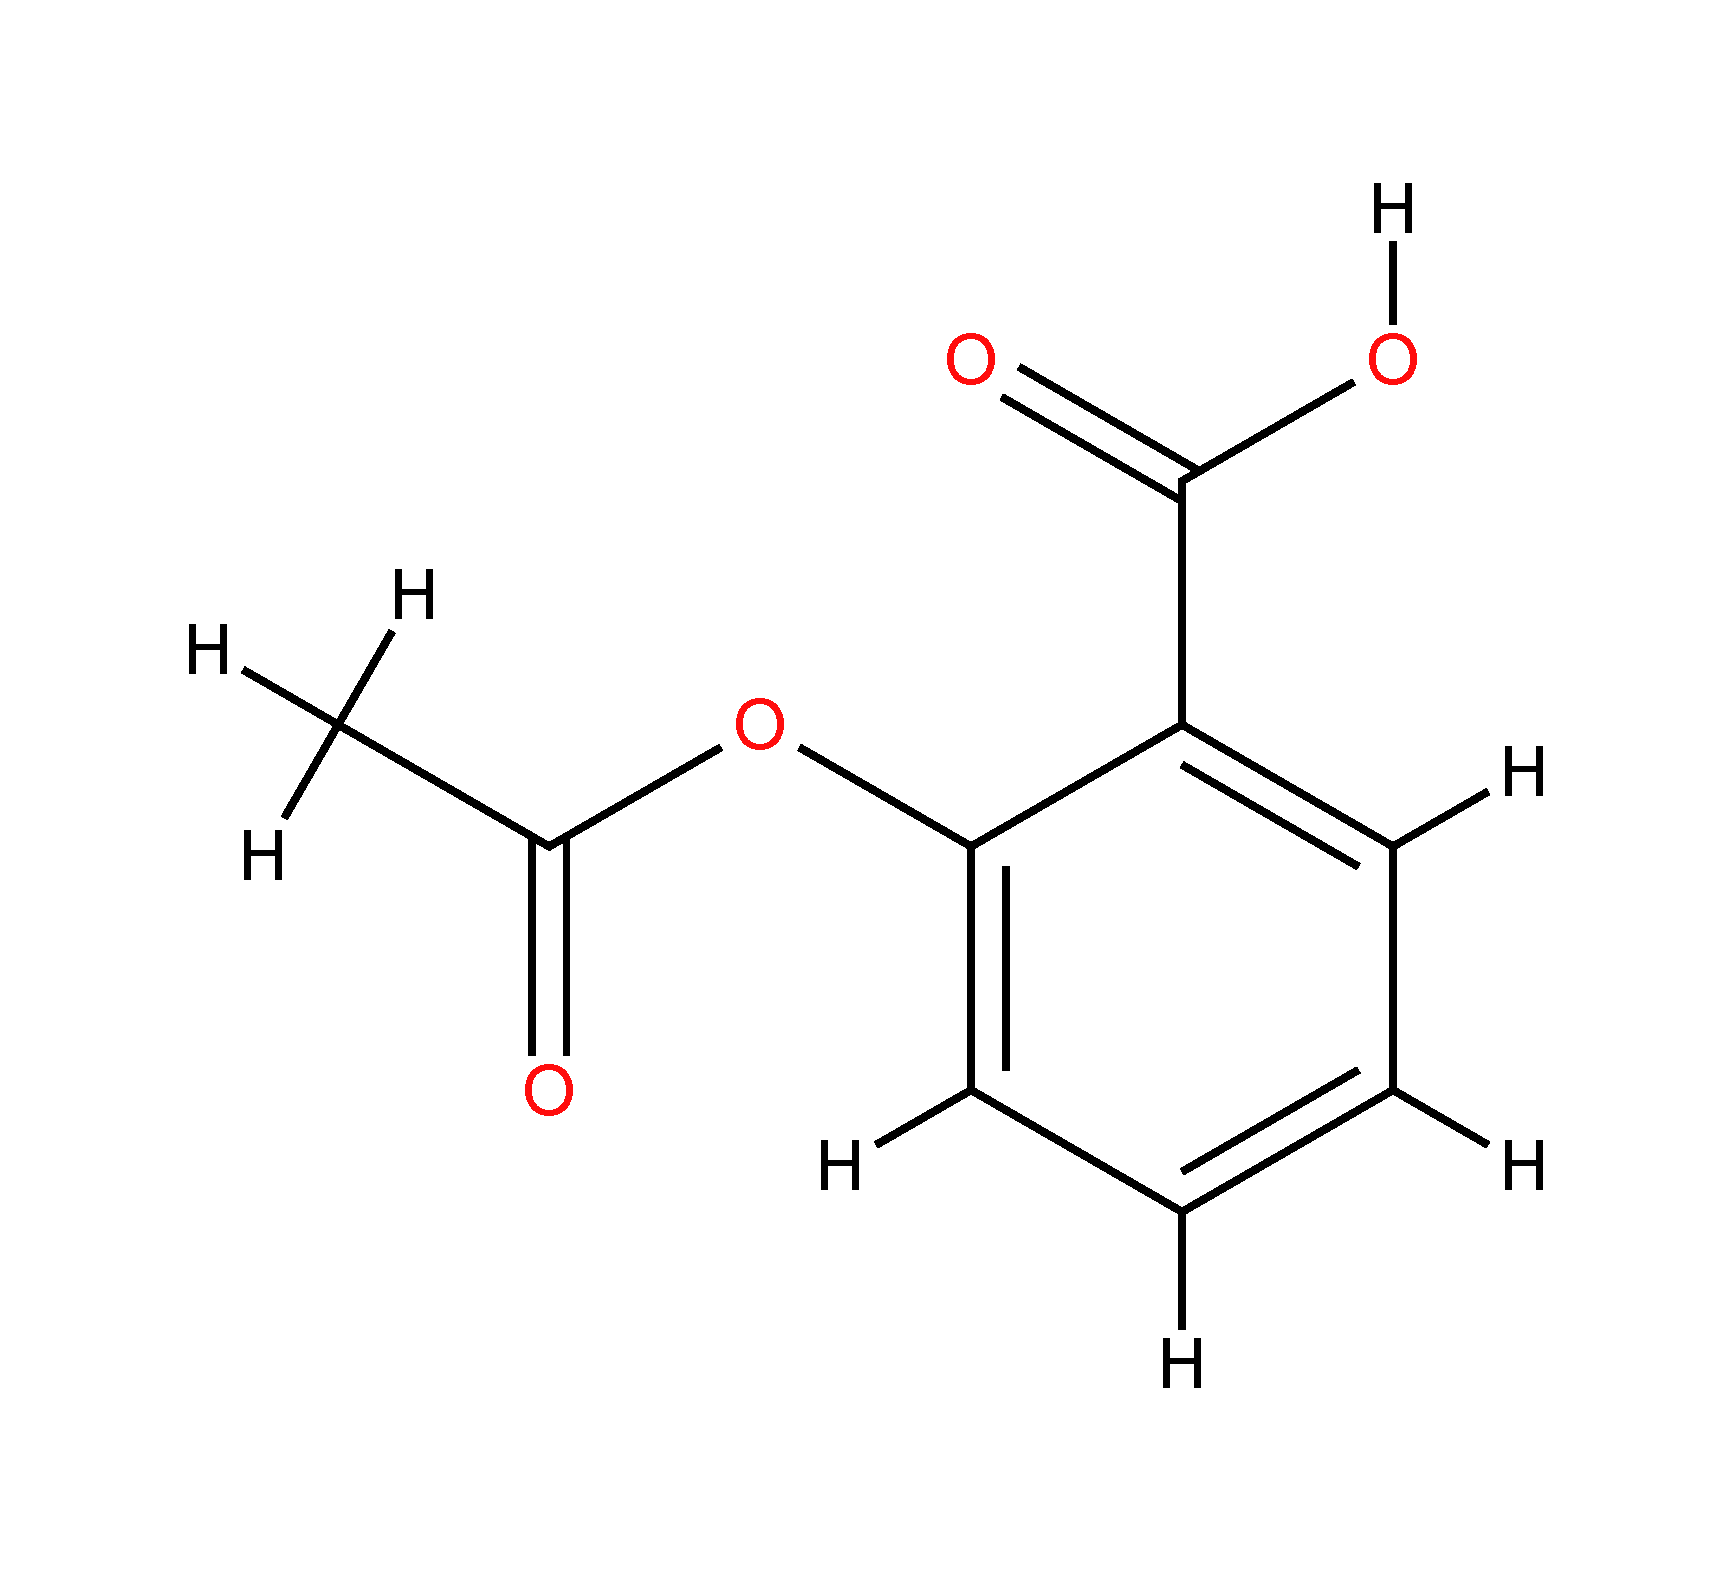
\includegraphics[width=0.25\textwidth]{img/aspirine.pdf}}
{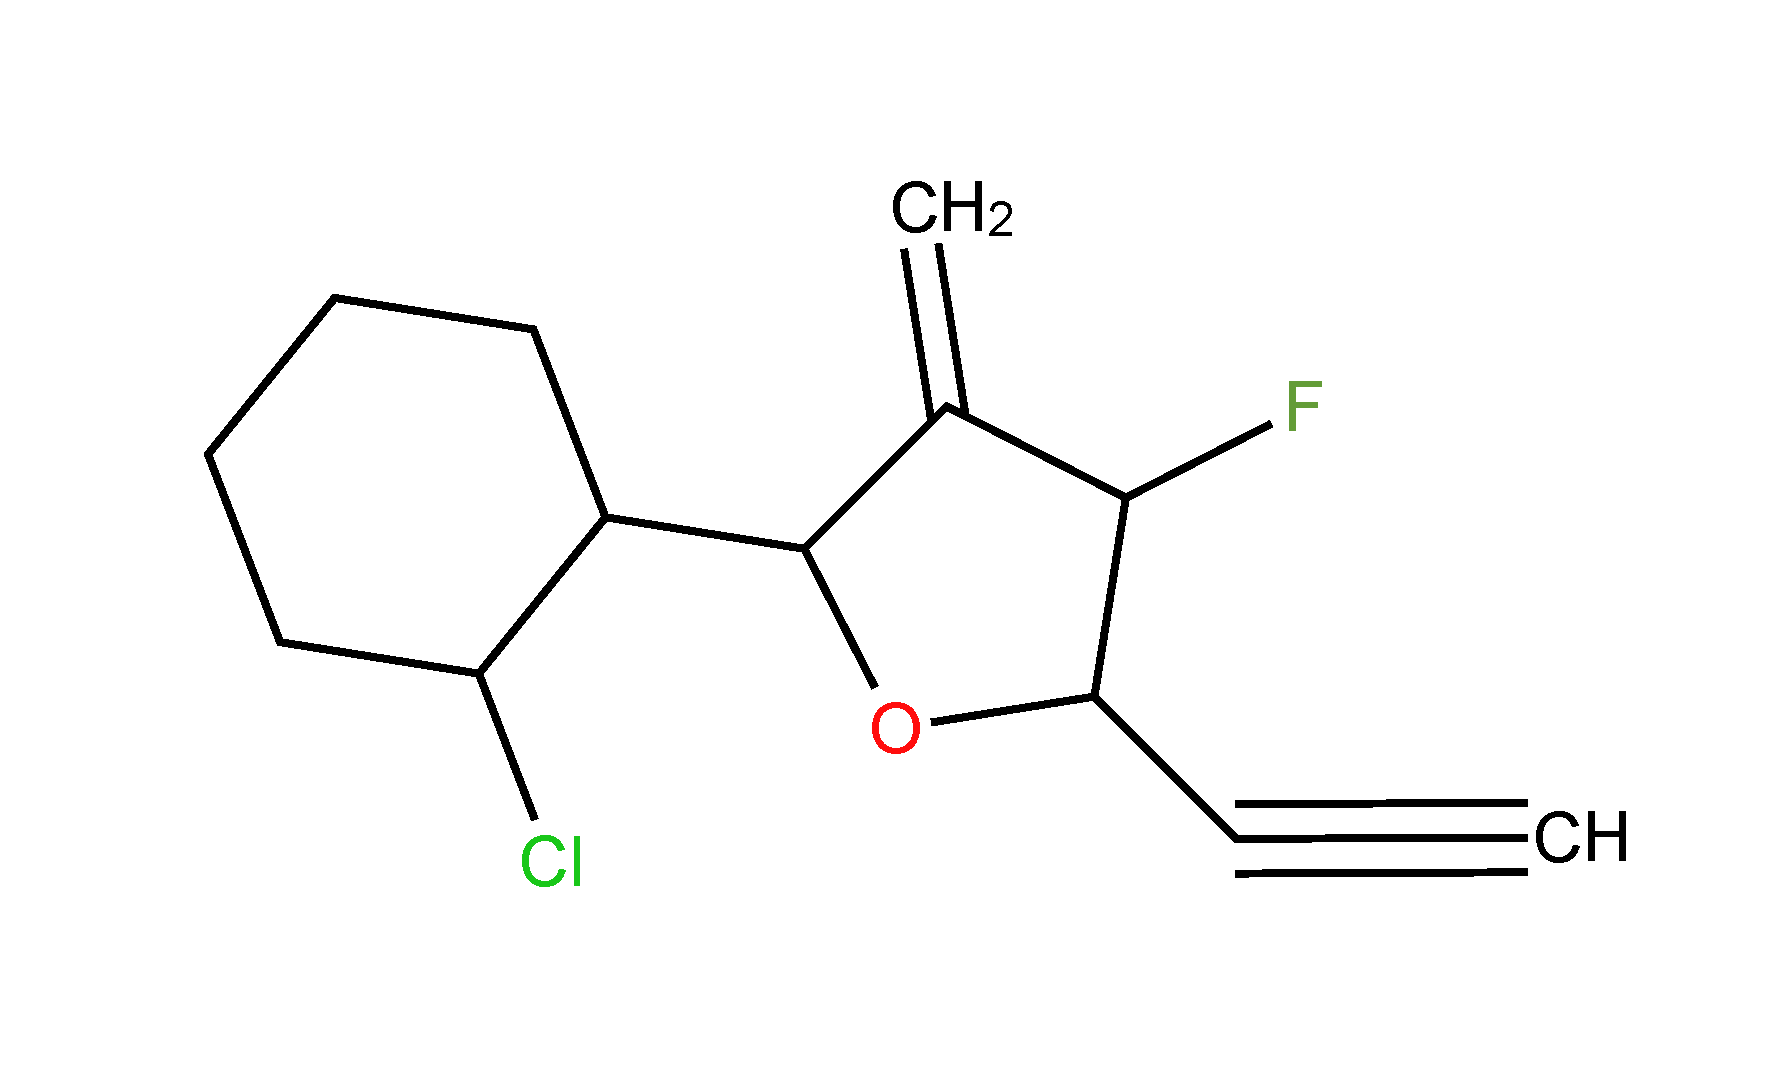
\includegraphics[width=0.35\textwidth]{img/1.pdf}}
\caption{Парацетамол, аспирин и нарисованная автором молекула}
\end{figure}

\noindent Для машинного представления разработано несколько форматов файлов. Например \begin{tt}{MDL Molfile}\end{tt} или 
\begin{tt}Daylight SMILES\end{tt}.

\begin{figure}[h]
\centering
{
\includegraphics[scale=0.8, clip, trim = 95mm 200mm 95mm 20mm]{img/benzene_smiles.pdf}}
{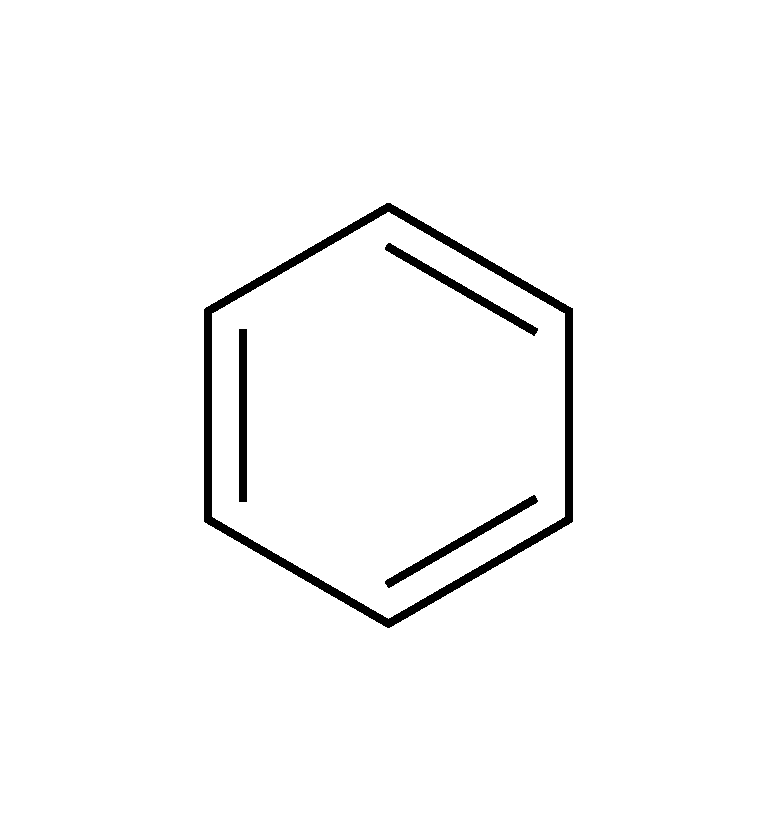
\includegraphics[scale=0.4, clip, trim = 25mm 10mm 25mm 10mm]{img/benzene.pdf}}
{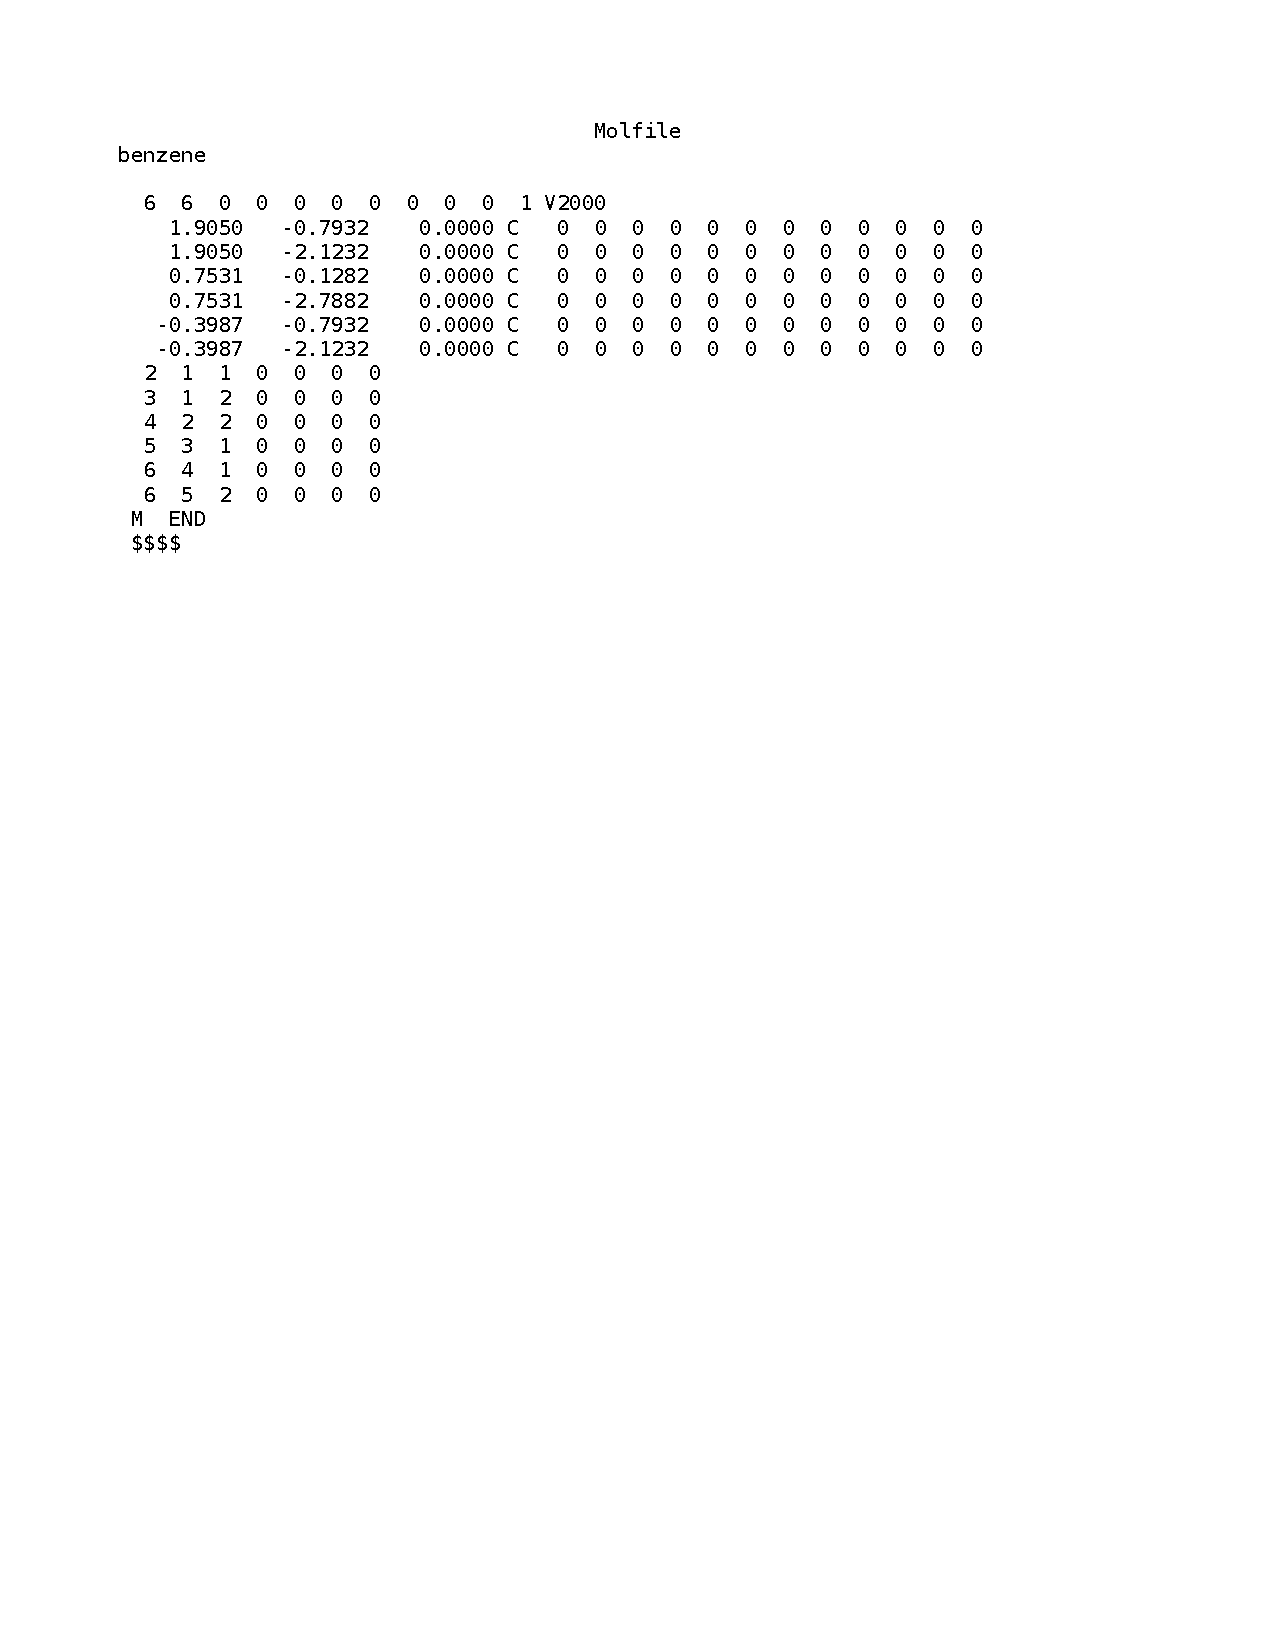
\includegraphics[scale=0.6, clip, trim = 10mm 180mm 45mm 10mm]{img/benzene_molfile.pdf}}
\caption{Бензол в машинном представлении}
\end{figure}

\noindent Вообразим: специалист изучает статью по химии, в которой есть изображения молекул, и в некоторый момент у него возникает 
потребность загрузить какую-то молекулу и поработать с ней с помощью имеющегося у него инструментария. Да, конечно,
вполне возможно просто перерисовать молекулу, используя редактор и затем сохранить её. Но что, если нужных молекул много? 
Или, если молекула одна, но она достаточно большая и её перерисовка займет много времени? \\ 

\noindent 
Здесь и может быть использовано распознавание изображений. Эта область искуственного интеллекта в некотором смысле ``обратна'' 
компьютерной графике. Если задача компьютерной графики визуализировать модель, в нашем случае отобразить молекулу, то задача 
распознавания изображений --- восстановить модель по картинке, то есть восстановить компьютерное представление молекулы. Или, 
если потребовать чуть большего, извлечь из статьи все молекулы. О более глобальном приложении распознавания химических структур 
можно прочесть в \cite{pavlov}.\\

\noindent
В рисунках молекул может присутствовать множество элементов, отображающих различные химические особенности соединений,
о распознавании двух из них я поведу речь далее. Надо сказать, что для распознавания не так уж важно, что элементы означают с точки 
зрения химии, куда важнее понять \emph{что} они являют собой на картинке, почему люди легко осознают, что это тот или 
иной элемент. И попытаться научить тому же самому компьютер. 

\onecolumn

\section{Задачи летней практики}
\noindent
Перед тем как перейти к описанию задач, которые мне довелось решать, приведу в общих чертах описание всего процесса распознавания.

\begin{codebox}
  \Procname{$\proc{Recognize(I)}$}
  \li \Comment Пусть $I$ --- картинка, а $M$ --- молекула, 
  \li машинное представление которой предстоит построить.
  \li $M = \varnothing $
  \li
  \li \Comment Для начала подвергнем картинку некоторой обработке.
  \li $\proc{ProcessFilters(I)}$
  \li
  \li \Comment Процедура суперсегментации пытается выделить на картинке 
  \li \Comment участок содержащий молекулу,
  \li \Comment далее будем работать с картинкой $I_{M}$.
  \li $ I_{M} = \proc{SuperSegmentation($I_{M}$)} $
  \li  
  \li \Comment Сегментация картинки это выделение отдельных компонент связности или сегментов. 
  \li \Comment $S$ --- хранилище сегментов.
  \li $ S = \proc{Segmentation(I)} $
  \li 
  \li \Comment Происходит извлечение из изображение стерео-вниз связей. Почему этот идет первым и
  \li \Comment как он происходит описано ниже. Это одна из задач практики.
  \li $ M \gets \proc{ExtractSingleDownBonds(S)} $
  \li
  \li \Comment Все сегменты разделяются на два слоя: символьный $L_{s}$ и графический $L_{g}$. 
  \li \Comment Побочным результатом выполнения этой процедуры является оценка высоты заглавной
  \li \Comment буквы, о чем подробнее можно будет прочесть ниже.
  \li $ L_{s}, L_{g} \gets \proc{Separation(S)} $
  \li 
  \li \Comment Буквы объединяются в группы и добавляются к молекуле, распознавание символов пока
  \li \Comment не происходило.
  \li $ M \gets \proc{ GetLabels($L_{s}$) } $
  \li
  \li \Comment Из графического слоя извлекаются кусочно-линейные элементы, строится скелет молекулы.
  \li \Comment Здесь же осуществляется поиск колец на картинке.
  \li $ M \gets \proc{ ExtractGraph($L_{g}$) } $
  \li
  \li \Comment Граф построен, информация о стерео-вверх связях должна быть восстановлена.
  \li $ M \gets \proc{FetchSingleUpBonds($I_{M}$)} $
  \li
  \li \Comment Пришло время для того чтобы распознать символы.
  \li $ \proc{RecognizeLabels(M)} $
  \li
  \li \Comment Осталось исправить или восстановить направления стерео-вниз связей и
  \li \Comment правильно обработать извлеченные ранее кольца.
  \li $ M \gets \proc{FixStereoCenters()} $
  \li $ \proc{Aromatize(M)} $
\end{codebox}

\noindent
Детально в этом отчете буду рассмотрены процедуры $\proc{ExtractSingleDownBonds}$, $\proc{FixStereoCenters}$ (см. \ref{subsec:stereobonds}), важная
составляющая процедуры $\proc{Separation}$ (см. \ref{subsec:capheight}), а также решение задачи извлечения колец, которое 
входит в процедуру $\proc{ExtractGraph}$ и последующая процедура применения знаний о кольцах $\proc{Aromatize}$ (см. \ref{subsec:rings}). Для 
подробных сведений о распознавании символов и извлечении кусочно-линейных элементов картинки, т.е. о процедурах $\proc{GetLabels}$, 
$\proc{RecognizeLabels}$, $\proc{ExtractGraph}$ следует обратиться к \cite{smolov} и \cite{zahn}. Также некоторые детали
$\proc{ProcessFilters}$ и $\proc{SuperSegmentation}$ будут обсуждаться в заключении (см. \ref{sec:future}). 


%TODO: this section
\subsection{Оценка высоты символа}
\label{subsec:capheight}

\noindent
Отделение графических и символьных данных базируется на знании некоторой оценки высоты заглавной буквы на картинке и представляет из себя
достаточно тривиальную процедуру классификации сегментов. Наибольший интерес представляет задача: как правильно оценить высоту символа. В
этом разделе под символом я буду понимать заглавную букву. \\

\noindent
Первое наблюдение о символах: символы представляют собой набор сегментов примерно одинаковой высоты, значение отношения ширины к высоте которых
находится в промежутке $[a;b]$, где $a$ и $b$ - опытно вычисленные константы. Алгоритм на основе такого критерия был реализован и 
сразу было выяснено, что под такой же критерий подпадают отдельно стоящие наклоненные отрезки связей. Например, части двойных связей. 
Следовательно, понадобилась вспомогательная процедура для проверки является ли сегмент отдельным отрезком.

\begin{codebox}
  \Procname{$\proc{IsSingleEdge(S)}$}
  \li \Comment Пусть $S$ - проверяемый сегмент
  \li
  \li \Comment Запомним плотность сегмента
  \li $density = \proc{Density(S)}$
  \li
  \li \Comment Применим утончающий фильтр
  \li $\proc{ApplyThinFilter(S)}$
  \li
  \li \Comment Нарисуем отрезок и проверим изменилась ли плотность
  \li $\proc{DrawLine(S, 0, 0, Width(S), Height(S)}$
  \li
  \li \If $|\frac{density}{\proc{Density(S)}}| < \varepsilon$
  \li \Then \Return \const{true} \End
  \li \Return \const{false}
\end{codebox}

\noindent
Под плотностью картинки понимается отношение количества черных пикселей к общему количеству пикселей. В случае, если сегмент являлся отрезком, то
после применения утончающего фильтра его толщина будет измеряться одним пикселем. Ясно, что после искуственной отрисовки отрезка в отфильтрованный 
сегмент его плотностью достаточно сильно упадет, что и позволит сделать вывод о том, являлся ли сегмент отрезком или нет. Метод может показаться
несколько кустарным, однако он достаточно хорошо продемонстрировал себя на практике. Для сведений об утончающих фильтрах можно обратится к 
\cite{gonzalez} (канонические алгоритмы на основе морфологических операций) и \cite{cychosz} (этот фильтр был реализован). \\

\noindent
Теперь, имея в арсенале процедуру $\proc{IsSingleEdge(S)}$ не сложно реализовать алгоритм оценки высоты символа.

\begin{codebox}
  \Procname{$\proc{EstimateCapHeight(H)}$}
  \li \Comment Пусть $H$ - массив высот сегментов
  \li
  \li \Comment Сгруппируем высоты, допуская отклонение на некоторую константу
  \li $ H_{g} = \proc{GroupByHeight(H)} $
  \li
  \li \Repeat 
  \li $ h_{g} = \proc{ LongestGroup($H_g$) } $
  \li \If $ \proc{CheckSequence($h_{g}$)} $
  \li \Then $cap\_height = \proc{InterQuartileMean($h_{g}$)} $
  \li \Return \End
  \li $\proc{Delete($h_{g}$)}$
  \li \Until \const{true} \End
\end{codebox}

\noindent
Главный цикл процедуры $\proc{EstimateCapHeight}$ рассматривает наборы высот, начиная с самого большого. Процедура $\proc{CheckSequence}$, с помощью
рассмотренной выше процедуры $\proc{IsSingleEdge}$ проверяет, есть ли в наборе хотя бы один не отрезок. В случае, если проверка проходит успешно,
за оценку высоты символа берется среднее набора. Интерквартальное среднее здесь показало наиболее точный результат. 

\subsection{Стереосвязи}
\label{subsec:stereobonds}

Как правило, обычную одинарную связь на рисунке молекулы изображают единичным отрезком. Однако порой важно знать расположение
отдельного атома относительно плоскости остальной молекулы, т.е. находится ли атом, или, может быть, часть молекулы выше или ниже. 
Для того чтобы отобразить такое расположение отдельного атом используют особый тип связи --- стереосвязь. Различают стерео-вниз 
(\emph{single down bond}) и стерео-вверх (\emph{single up bond}). В мои задачи входило распознавание стерео-вниз связей. \\

\noindent
Исходя из наблюдений и согласуя их со стандартом отрисовки молекул (см. \cite{iupac}), я сформулировал критерий интересующих меня
элементов. Стерео-вниз связь --- это набор из $k$, где $k \ge 3$, параллельных друг другу отрезков. При этом расстояние между
соседними отрезками примерно одинаковое. Критерий, как видно, конструктивен и из него был немедленно извлечен алгоритм.  

%TODO: this figure

%\begin{SCfigure}
%\centering
%{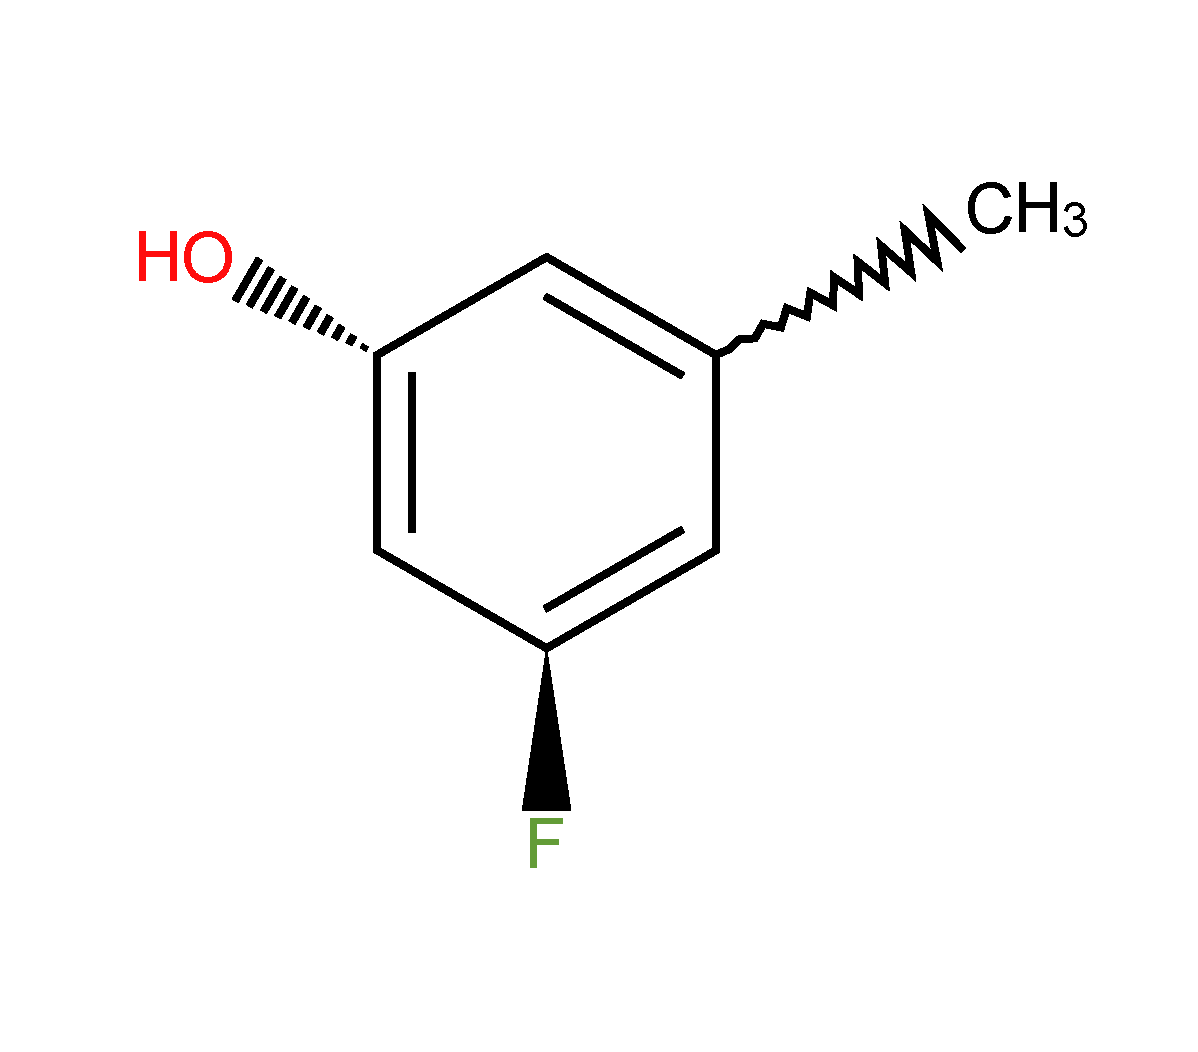
\includegraphics[scale=0.4, clip, trim = 15mm 10mm 15mm 10mm]{img/stereo.pdf}}
%\caption{Закрашенный треугольник означает, что атом фтора находится ближе к обозревателю, это стерео-вверх связь. 
%Треугольник, состоящий из параллельных отрезков говорит о том, что атом кислорода лежит за плоскостью картинки --- стерео-вниз связь.}
%\end{SCfigure} 

\begin{codebox}
  \Procname{\proc{ExtractSingleDownBonds}$(S)$}
  \li \Comment $Q$ --- хранилище одиночных отрезков
  \li $Q = \varnothing$
  \li
  \li \Comment $S$ --- хранилище сегментов картинки  
  \li \For $s \in S$ 	
  \li \Do \If \proc{IsSingleEdge}$(s)$
  \li   	\Then $Q \gets s$
  \li \End \End
  \li \Comment Все отрезки найдены, можно приступать к извлечению связей
  \li \For $a \in Q$
  \li \Do $L_{a} = \emptyset $ 
  \li \For $b \in Q, b \ne a$ 
  \li \Do \If $ a \parallel b $
  \li \Then $L_{a} \gets b$
  \li \End \End 
  \li \Comment Теперь в $L_{a}$ все отрезки параллельные $a$, осталось проверить расстояние
  \li \If \proc{CheckDistance}$(L_{a})$
  \li \Then \proc{AddSingleDownBond}$(L_{a})$
  \li \Comment Отрезки составили связь, больше они не понадобятся и будут только мешать
  \li \proc{DeleteSegments}$(L_{a})$
\end{codebox}

\noindent
Сегмент --- компонент связности картинки. Ясно, что в $L_{a}$ может оказаться не одна связь, за этим следит функция \proc{CheckDistance}, выбирая
из набора параллельных отрезков, наборы с одинаковым расстояниями между соседними отрезками. Функция \proc{AddSingleDownBond} определяет
координаты начала и конца связи, а также её направление, затем добавляет в конструирующийся граф. Направление связи можно определить, узнав
какой из двух крайних отрезков длиннее. Однако встретились такие рисунки, где стерео-вниз связи были изображены отрезками по длине одинаковыми.
Казалось, что такой способ отрисовки вносит путаницу, на самом же деле это не так. Здесь пригодились некоторые сведения из химии: дело в том, что
существует конечный набор корректных конфигураций стереосвязей. Применение этих сведений требует знаний о том, какие атомы соединены стереосвязями,
какие еще связи у атома. Следовательно, этот этап отложен до момента, когда граф молекулы уже почти построен.  


\subsection{Ароматичные кольца}
\label{subsec:rings}

%TODO: rewrite
Существуют в химии понятия \emph{ароматичность}, ароматичная связь (\emph{aromatic bond}). Если в рисунке молекулы находится выпуклый 
многоугольник, целиком состоящий из ароматичных связей, то принято не изображать отдельно связи, а рисовать окружность внутри такого многоугольника.

%TODO: this figure
\begin{figure}[h]
\centering
{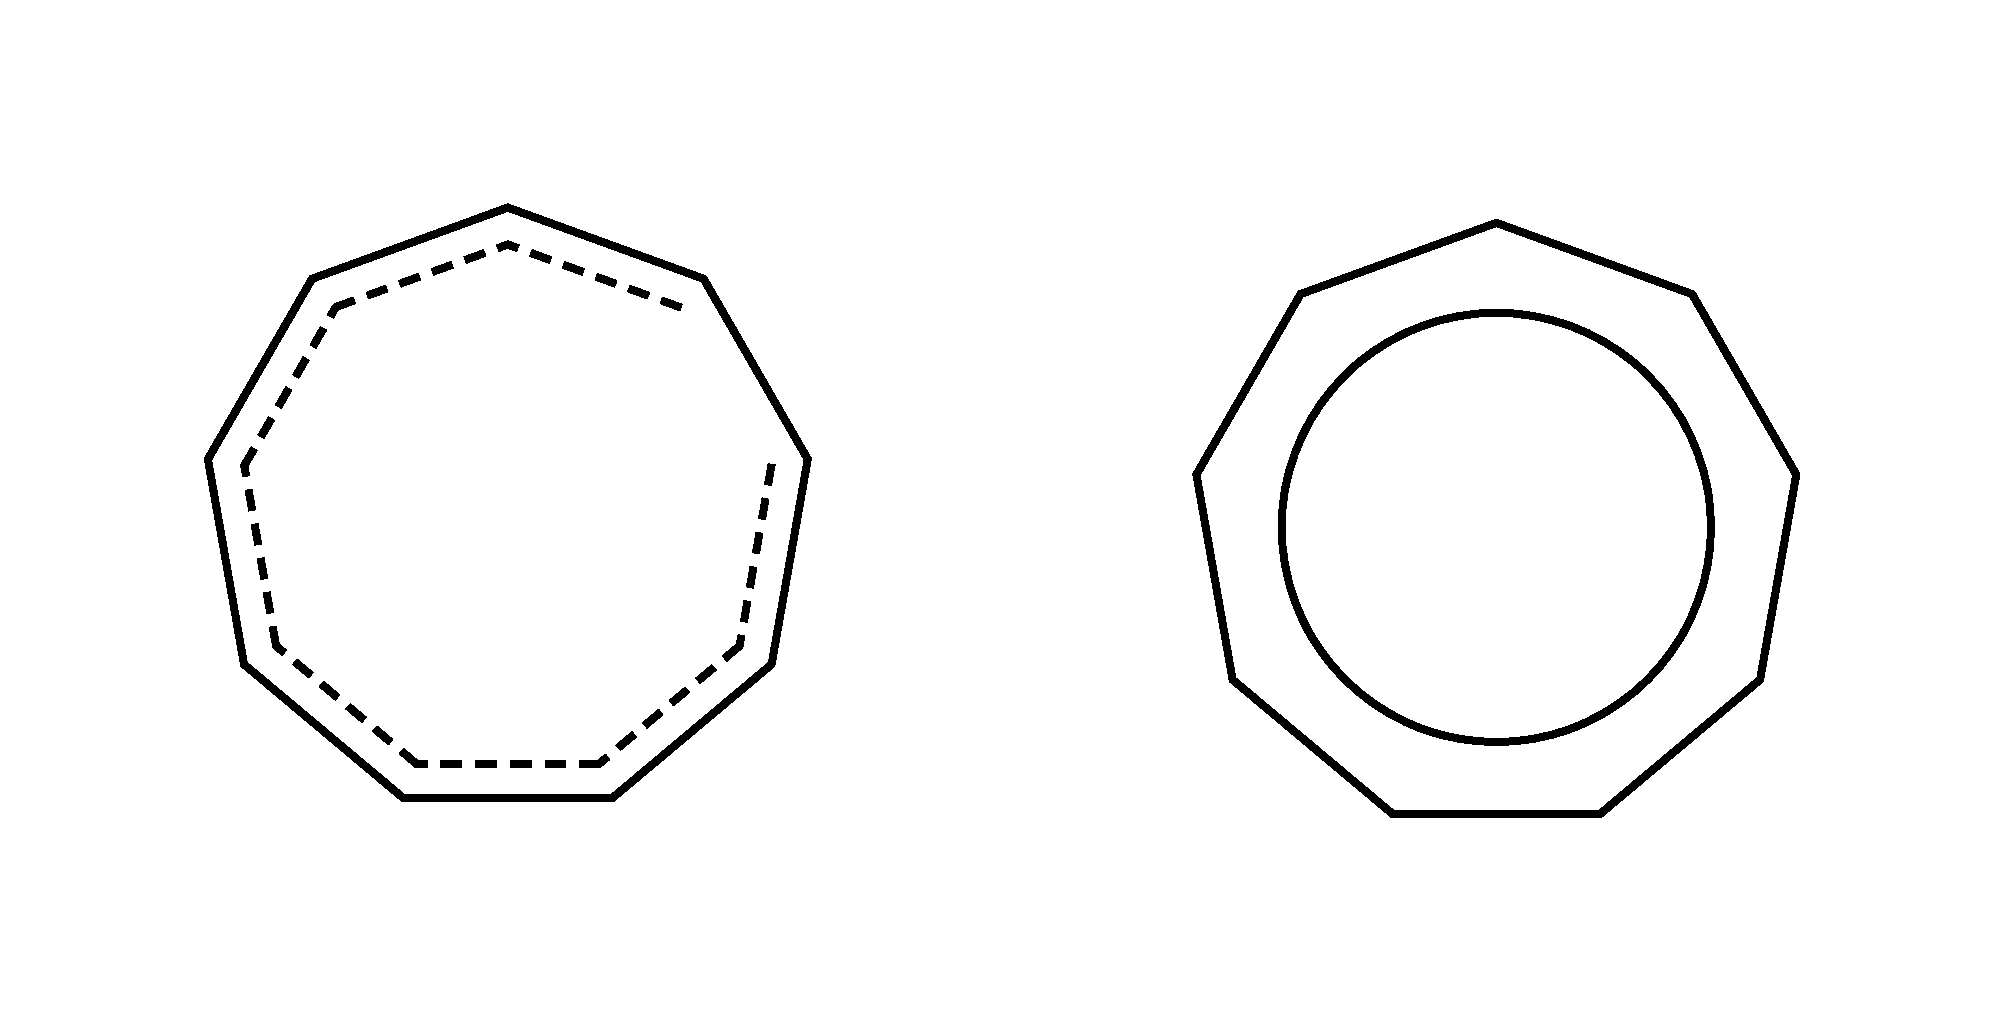
\includegraphics[scale=0.4, clip, trim = 32mm 32mm 35mm 35mm]{img/rings.pdf}}
\caption{Ароматичные связи изображают двумя параллельным линиями: сплошной и пунктирной. Молекула справа получается из молекулы слева добавлением
недостающей ароматической связи.}
\end{figure}

\noindent
Возникает задача, которую сразу можно разбить на две подзадачи: необходимо найти на рисунке окружности, а затем пометить соответствующие связи
как ароматичные. Как и в случае со стереосвязями, упомяну, в какой момент должны распознаваться кольца: извлечение колец должно происходить после того, 
как из картинки уже были удалены все символьные данные и это хорошо, так как буквы \emph{O} могли бы ошибочно отсеяться. \\

\noindent
Для решения первой задачи я воспользовался тем, что в проекте уже успешно работало: распознаванием символов, которое основано на подсчете 
\emph{дескрипторов Фурье}.

\begin{codebox}
  \Procname{\proc{FindCircles}$(S)$}
  \li \Comment Пусть $I$ - пустая картинка, $Q$ - хранилище колец, а $S$ - хранилище сегментов картинки
  \li $I = \varnothing$
  \li $Q = \varnothing$
  \li \Comment Рисуем в $I$ окружность и считаем дескрипторы
  \li $\proc{PutCircle}(I)$
  \li $ FD_{c} = \proc{GetFourierDescriptors}(I)$
  \li \Comment Далее ищем похожие сегменты
  \li \For $s \in S$
  \li \Do $FD_{s} = \proc{GetFourierDescriptors}(s)$
  \li \If $ | \parallel FD_{s} \parallel - \parallel FD_{c} \parallel |  < \varepsilon $
  \li \Then $Q \gets s$  
\end{codebox}

\noindent
Подсчет дескрипторов --- процедура не слишком быстрая и приведенный выше алгоритм можно ускорить, рассматривая только сегменты
с отношением ширины к высоте близким к единице, то есть квадратные сегменты. Теперь, когда все кольца извлечены, осталось подождать, пока
будет построен граф; связи, из которых состоят многоугольники, будут помечены как одинарные --- внесём правки.

\begin{codebox}
  \Procname{$\proc{Aromatize}(G)$}
  \li \For $q \in Q$
  \li \Comment Для каждого кольца $q$ находим ближайшую к нему связь
  \li \Do $b = \proc{FindClosestBond}(q)$
  \li $begin\_vertex = b.end$
  \li $current\_vertex = begin\_vertex$
  \li $distance = \infty$
  \li \Comment Обходим многоугольник и помечаем связи 
  \li \Repeat 
  \li \For $v \in Adj(current\_vertex)$
  \li \Do \If $\proc{Distance}(Bond(v,current\_vertex), q) < distance $
  \li \Then $distance = \proc{Distance}(Bond(v,current\_vertex), q)$ 
  \li $next\_vertex = v $ \End \End
  \li $\proc{SetAromatic}(Bond(current\_vertex, next\_vertex))$
  \li $current\_vertex = next\_vertex$ \
  \li \Until $current\_vertex \ne begin\_vertex$
\end{codebox}

\noindent
Обход многоугольника осуществляется с естественной эвристикой: нет нужды далеко отходить от кольца. \\ 
\noindent
Подробнее о распознавании символов
и дескрипторах Фурье можно прочесть в \cite{smolov} и \cite{zahn}. Отмечу также, что для поиска окружностей существует известные методы, 
например преобразование Хафа (см. \cite{gonzalez}). %TODO: Hough transform

%TODO: 

\section{Заключение}
\label{sec:future}

Не надо долго думать, чтобы понять как много вопросов и нерешенных сложных задач возникает в распознавании химических структур. Как
правильно разобрать картинку, в которой содержится не одна молекула, содержится реакция, таблица заместителей? Как вообще
найти изображение именно молекулы в статье? Как правильно обработать слипшиеся символы, слипшуюся связь и символ? Что касается задач, изложенных
в этом отчете, то я бы сказал, что решены они были с точностью $\varepsilon$, как это обычно и бывает в распознавании изображений: остаются
кольца, у которых дескрипторы не совпадут (например на картинках плохого качества после сканирования), отрезки, которые не войдут в стереосвязи.

\section{Замечания}

Проект собирался под операционные системы \begin{tt}Linux, Windows\end{tt} и \begin{tt}Mac OS X\end{tt} обеих, распространненных ныне разрядностей.
Разработка велась с помощью \begin{tt}Microsoft Visual Studio 2008\end{tt} и \begin{tt}NetBeans 6.8\end{tt} на языке \begin{tt}C++\end{tt}, 
для сборки была выбрана программа \begin{tt}scons,\end{tt} для контроля версий --- \begin{tt}Subversion.\end{tt} Отчет был подготовлен в 
текстовом редакторе \begin{tt}vim\end{tt} с использованием \begin{tt}\LaTeX\end{tt}, иллюстрации в векторном виде подготовлены с помощью программ 
\begin{tt}Dingo\end{tt} и \begin{tt}Ketcher\end{tt}, в некоторых местах использовался \begin{tt}OpenOffice\end{tt}. Титульная страница 
взята из \cite[стр.26]{gluhov}. Все указанные программы могут быть свободно загружены в интернете (\begin{tt}Visual Studio\end{tt} может быть
загружена в редакции \begin{tt}Express\end{tt}).

\begin{thebibliography}{9}

\bibitem{pavlov}
  Дмитрий Павлов,
  \emph{Навигация в мире органических соединений}.\\
  \url{http://shmat-razum.blogspot.com/2010/07/blog-post.html}

\bibitem{smolov}
  Виктор Смолов,
  \emph{Отчет по производственной практике}, СПБГПУ, кафедра <<Прикладная математика>>, 2010

\bibitem{iupac}
  \emph{Graphical Representation Standards For Chemical Structure Diagrams \\ (IUPAC Recommendations 2008)} \\
  \url{http://www.iupac.org/publications/pac/80/2/0277/}

\bibitem{gluhov}
  \emph{Правила оформления студенческих выпускных работ и отчетов. Положение.} 
  Под ред. В.В.Глухова.
  СПБ.:СПБГТУ, 1998

\bibitem{gonzalez}
  Gonzalez \& Woods,
  \emph{Digital Image Processing}, 2002

\bibitem{zahn}
  Charles T. Zahn \& Ralph Z. Roskies,
  \emph{Fourier Descriptors for Plane Closed Curves},
   IEEE Transactions on computers, Vol. c-21, No. 3, march 1972

\bibitem{cychosz}
  Joseph M. Cychosz,
  \emph{"Efficient Binary Image Thinning using Neighborhood Maps"}
  Graphics Gems IV, Academic Press, 1994

\end{thebibliography}

\end{document}

